% Technical Background, continuation of sec:tech-glmi (01_glm.tex): the generalised linear
% mixed model, the likelihood ratio test and the cluster risk. Created 2026-11-18 (user chose "New file +
% GLMM parts"): copied from the end of 01_mixed_model.tex (from "Clustered Outcomes and the Random
% Intercept"), which is no longer input but kept for its study notes and history. Labels unchanged
% (sec:tech-random-intercept, eq:tech-glmm, sec:tech-glmm-likelihood, eq:tech-lr, sec:tech-aggregation,
% eq:tech-agg-conditional), so Methods 05 and Appendix C keep pointing right.
% Edits on copying: "covariate" -> "feature" (user, 2026-11-18); the unit cumulative hazard Lambda_ij ->
%   H_ij, to match H(t) of 01_glm.tex and Figure 4.3 (H_i = sum_j H_ij reads naturally).
% Not yet rewritten in the plain register of 01_glm.tex. Citations as in 01_mixed_model.tex
%   (dobson2002glm, austin2017mhr), which that file records as checked.
% 2026-11-18 (user: "make glmm into a section on its own and glm on its own"): the subsection
%   "Clustered Outcomes and the Random Intercept" became the body of the new section Generalised Linear
%   Mixed Models (sec:tech-glmm); its label sec:tech-random-intercept now sits on the section, and
%   sec:tech-model moved here from 01_glm.tex, since Methods 05 uses it for the GLMM.
% 2026-11-18: rewritten in the register of 01_glm.tex around Figures 05 (fig:tech-glmm-frailty) and 06
%   (fig:tech-glmm-marginal), following the user's explanation of Figure 06 (where b comes from, what the
%   fit gives, the averaged risk of a new cluster, conditional vs marginal). sigma^2 -> sigma_b^2 to match
%   the figures; the two stale \todonote figure plans removed; all labels kept. New: eq:tech-glmm-pbar.
%   eta_ij stays the fixed part without b_i (Methods 05, Appendix C). Figure 05's panel title writes
%   eta_i including b_i: align illus_random_intercept.py if wanted.
% CHECK (uncited reasoning, new 2026-11-18): sigma_b is learned from how strongly events group within
%   clusters; the marginal risk differs from the risk at b = 0 because p(b) is curved (Appendix C cites
%   pavlou2015marginal, skrondal2009prediction for this point; check before citing here).
% 2026-11-18 (user: "a little too much, look at how glm does it"): shortened to the pattern of
%   01_glm.tex: short paragraphs, equations inside sentences, figures pointed to in brackets, captions
%   "Illustration of ..., showing ...". Panel-by-panel narration and the GLM-vs-GLMM closer cut.
% 2026-11-18 (user: GLMM is used for curvature only, which varies within and between persons): the
%   conditional-reading paragraph no longer says a within-cluster feature gives a within-cluster
%   comparison. The estimate mixes within- and between-cluster comparisons and assumes they agree (root
%   CLAUDE.md: "beta mixes between- and within-person information"). Uncited; CHECK for a source on
%   within/between effects in random-intercept models (e.g. Neuhaus and Kalbfleisch 1998, not opened).
%   The between-cluster sentence stays for the risk factors, constant within a person.
% 2026-11-18 (user: "move this to methodology, it is a special case of the use of hazard models"): the
%   cluster-risk paragraph (sec:tech-aggregation, eq:tech-agg-conditional, dilution) moved to Methods 05,
%   sec:method-added-value, as eq:method-agg-conditional. Subsection renamed "Likelihood Ratio Test".
% 2026-11-18 (user agreed): the likelihood ratio test moved to 01_glm.tex (sec:tech-lr, with eq:tech-lr), since
%   the bifurcation GLM uses it too. Here only the averaged likelihood and the dependence assumption
%   remain, as the closing paragraph of 4.2 under the kept label sec:tech-glmm-likelihood; subsection
%   4.2.1 removed. Dobson Sec. 11.7 kept for the GLMM use, Sec. 5.7 moved with the test.
% Open: Appendix B (link_choice.tex) still writes the cumulative hazard as Lambda_i.
% 2026-11-18 (user: two models, a GLMM for curvature and a person-level GLM for the angle and asymmetry):
%   one sentence added in sec:tech-glmm-likelihood saying a GLM is also fitted by maximum likelihood, without
%   the average over b, and that the LR test applies to both, since Methods 05 tests the GLM with eq:tech-lr.
%   CHECK: uncited; dobson2002glm Sec. 5.7 (already cited for eq:tech-lr) covers the GLM case. Confirm when
%   the Dobson PDF is opened.

\section{Generalised Linear Mixed Models}
\label{sec:tech-glmm}
\label{sec:tech-model}
\label{sec:tech-random-intercept}

The GLM treats all outcomes as independent \cite[Section~3.4]{dobson2002glm}. This does
not hold when units are grouped into clusters, such as several observations of the same person. Units
of the same cluster share traits that the features do not capture, so their outcomes are correlated,
and a model that ignores this gives invalid inference \cite[Section~11.1]{dobson2002glm}. A generalised linear mixed model (GLMM) accounts for this by adding
a random intercept $b_i$ for each cluster to the linear predictor \cite[Section~11.5]{dobson2002glm}.
With $i$ now indexing the cluster and $j$ the unit within it, the risk becomes
\begin{equation}
  p_{ij}(b_i) = 1 - \exp\{-\exp(\eta_{ij} + b_i)\},
  \qquad
  b_i \sim \mathcal{N}(0, \sigma_b^2).
  \label{eq:tech-glmm}
\end{equation}
The coefficients $\beta_k$ are shared by all clusters and are referred to as fixed effects, while $b_i$
is referred to as a random effect.

The random intercept shifts the linear predictor of every unit in the cluster, which multiplies its
hazard by $\exp(b_i)$, referred to as the frailty of the cluster (Figure~\ref{fig:tech-glmm-frailty})
\cite[Section~2.2]{austin2017mhr}. Clusters with the same features can therefore have different risks.
How much the frailty varies between clusters is summarised by the median hazard ratio (MHR). It is the
median ratio between the hazards of two units with the same features from two randomly chosen
clusters, with the higher hazard divided by the lower \cite[Section~2.2]{austin2017mhr}.

\begin{figure}[tbp]
  \centering
  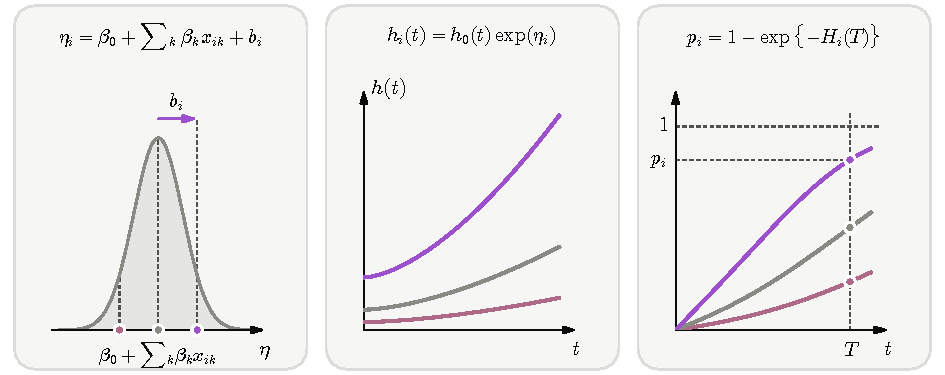
\includegraphics[width=\textwidth]{content/technical/figures/05_illus_random_intercept.pdf}
  \caption{Illustration of the random intercept for three clusters with the same features, showing
  how $b_i$ shifts the linear predictor (left), multiplies the hazard (middle) and changes the risk by
  time $T$ (right).}
  \label{fig:tech-glmm-frailty}
\end{figure}

The individual $b_i$ are never observed. The model instead estimates their standard deviation
$\sigma_b$ from how strongly the events group within clusters (Figure~\ref{fig:tech-glmm-marginal},
left and middle). For a new cluster $b_i$ is unknown, so its risk is averaged over the fitted
distribution (Figure~\ref{fig:tech-glmm-marginal}, right),
\begin{equation}
  \bar p = \int p(b)\,\phi(b)\,\mathrm{d}b,
  \label{eq:tech-glmm-pbar}
\end{equation}
where $\phi$ is the density of $\mathcal{N}(0, \hat\sigma_b^2)$. The result is referred to as the
marginal risk. Since $p(b)$ is curved, it differs from the risk at $b = 0$.

\begin{figure}[tbp]
  \centering
  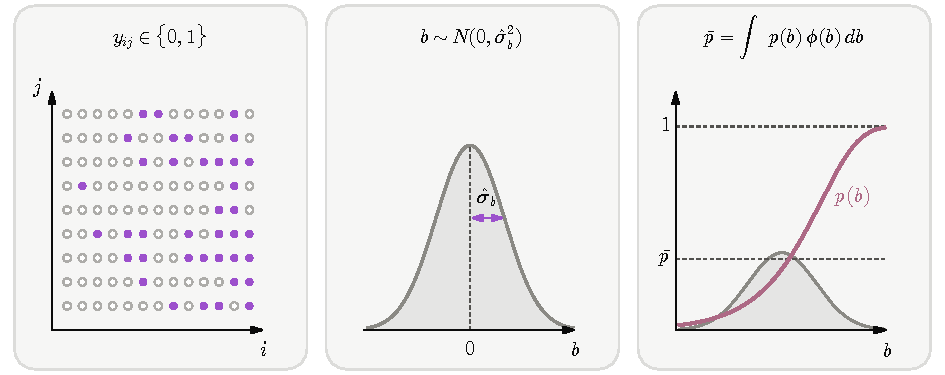
\includegraphics[width=\textwidth]{content/technical/figures/06_illus_random_intercept_integration.pdf}
  \caption{Illustration of how the random intercept is estimated and used, showing events grouped
  within clusters (left), the fitted distribution of the random intercepts (middle) and the risk of a
  new cluster averaged over that distribution (right).}
  \label{fig:tech-glmm-marginal}
\end{figure}

The hazard ratios $\exp(\beta_k)$, in contrast, are conditional on $b_i$ and compare units with the
same random intercept. For a feature that varies within clusters, the estimate draws on two kinds of
comparison, between units of the same cluster and between clusters, and the model assumes that both
give the same hazard ratio. 

\label{sec:tech-glmm-likelihood}%
The fixed effects and $\sigma_b$ are also estimated by maximum likelihood. The random intercepts are
not observed, so the likelihood is averaged over their distribution, in the same way as the risk in
Figure~\ref{fig:tech-glmm-marginal} (Appendix~\ref{app:glmm-fitting}). Two such fits are compared with
the likelihood ratio test of Section~\ref{sec:tech-lr} \cite[Section~11.7]{dobson2002glm}. Its
reference distribution then assumes that the random intercept captures the dependence within clusters.
When some units of a cluster are more alike than others, a second random effect can be added for that
subgroup (Appendix~\ref{app:glmm-variance}).
